\subsubsection{Supramolecular Functional Materials and Metalloenyzme Models} 
\index{Nau, Werner}

\paragraph{Research Team}
Werner Nau (Professor), Mara Florea (Graduate Student), Andreas Hennig (PhD Student), Apurba Koner (PhD Student), Roland Meyer (PhD Student), Harekrushna Sahoo (Ph.D. in November 2006, later Postdoc), Thomas Schwarzlose (Scientific Research Assistant), Hamdy El- Sheshtawy (PhD Student), Vanya Uzunova (Graduate Student), Roy D�Souza (Graduate Student) \\


Supramolecular assemblies are composed of several molecular entities held together by weak intermolecular interactions. By rational selection of the components, nanomolecular materials with functional properties can be designed. For example, large macrocyclic host molecules with concave cavities can accommodate organic molecules as guests. If the selected guest molecule possesses additional receptor sites, e.g., for cations, and if a fluorescent molecule is selected as guest, fluorescent sensors for cations can be constructed. To by-pass the need for organic solvents, and to enable biological or environmental applications, it is generally desirable to select water-soluble host molecules, e.g., cyclodextrins, calixarenes, and cucurbiturils.\\
We are constructing photonic devices based on supramolecular architectures, fluorescent sensor systems for analytes, and metalloenzyme models. These have applications, among others, for fluorescence imaging, dye lasers, information storage, detection of trace elements, and bioassays, for example to detect neurotransmitters.



\paragraph{Highlights}

Macrocyclic host molecules have long been recognized as enzyme models. In 2006, we have communicated a conceptually novel but exceptionally simple supramolecular approach to metalloenzyme models in aqueous solution. It is based on the dynamic self-assembly between macrocyclic hosts with cation receptor properties, organic guests, and metal ions (see publication \cite{Nau9}). In the resulting ternary complex, the guest is held in place by hydrophobic interactions with the host, while the metal ion experiences attractive Coulombic interactions with the negative charges positioned at the portal of the macrocycle. We have examined the resulting ternary complexes both in aqueous solution, where functional aspects are of prime interest, as well as in the solid state, where structural aspects can be studied in detail. Figure \ref{fig:nau_nano} shows the structures of the ternary complexes based on 2,3-diazabicyclo[2.2.2]oct-2-ene as guest included in the cavity of \textit{p}-sulfonatocalix[4]arene as macrocyclic host and capped by transition metal ions as third component.\\
%
The close investigation of these complexes has allowed us to scrutinize the phenomenon of ``host-assisted metal-ligand bond formation'', because the complex between guest (inside the cavity) and metal ion (the lid on the upper rim, see Figure \ref{fig:nau_nano}) is only formed in the presence of the macrocyclic host. In addition, we observed a fascinating interplay between cooperative and competitive binding, which infers a striking selectivity for the formation of the ternary complexes as a consequence of a triple recognition pattern. Finally, based on the same working principle, we were able to use metal ions as enhancers in fluorescent sensor applications based on host-guest complexes; in this manner, a refined sensor for acetylcholine could be constructed (see publication \cite{Nau9}), which further improved the sensitivity of this supramolecular neurotransmitter sensor just introduced in the same year (see publication \cite{Nau1}).

\begin{figure}[ht]
  \begin{center}
   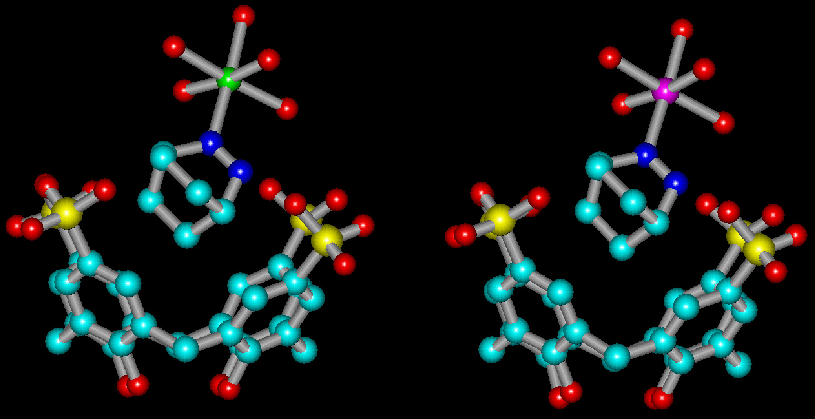
\includegraphics[width=\hsize]{Nau/Report-Nau-Nano.pdf}
    \mycaption{Crystal structures of the ternary complexes between 2,3-diazabicyclo[2.2.2]oct-2-ene, p-sulfonatocalix[4]arene, and transition metals, namely for $\mbox{Zn}^{\mbox{{\footnotesize 2+}}}$, in green, left, and for $\mbox{Co}^{\mbox{{\footnotesize 2+}}}$, in magenta, right; in collaboration with Prof. Ulrich Kortz and Dr. Mike Dickman, IUB.}\label{fig:nau_nano}
   \end{center}
\end{figure}

In addition, we have investigated in 2006 host-assisted $\mbox{p\textit{K}}_{\mbox{{\footnotesize a}}}$ shifts (see publications \cite{Nau3} and \cite{Nau6}), which we plan to elaborate on during the next years. We have also authored a concept article in \textit{Supramolecular Chemistry}, in which we introduce a new assay principle, which we referred to as protolytic displacement assays (see publication \cite{Nau12}); these assays exploit the previously observed $\mbox{p\textit{K}}_{\mbox{{\footnotesize a}}}$ shifts accompanying host-guest complexation for sensing purposes. Finally, we have been able to develop a high efficiency ``green'' dye laser based the use of rhodamine 6G in aqueous solution (see publication \cite{Nau14}). This dye laser by-passes for the first time the use of organic solvents, and instead employs water as environmentally benign and explosion-safe solvent. This application is made possible by the addition of cucurbit[7]uril as a supramolecular stabilizer. The new line of dye laser has the added advantage of an improved photostability and beam shape, which is the result of the advantageous thermo-optical properties of water as laser medium.\\
Additional applications of macrocyclic hosts deal with their effects on enzymatic activity, which will be described separately.\newline \newline Werner Nau is also involved in ``Bioassay Development and Biopolymer Dynamics and Structur''.



%Pictures are to be included via:



\paragraph{Collaborations}
Bremen Area Collaborations:
\begin{enumerate}
\item {\sl Jacobs University Bremen} \\ Prof. K. Brix \\ Dye Stabilization in Live Cells
\item {\sl Jacobs University Bremen} \\ Prof. A. Jeltsch \\ Investigation of Peptide Dynamics
\item {\sl Jacobs University Bremen} \\ Prof. U. Kortz and Dr. M. Dickman \\ Structural Investigations in Host-Guest Chemistry
\item {\sl Jacobs University Bremen} \\ Prof. R. Richards \\Hybrid Materials based on Cucurbiturils and Silver and Gold Nanoparticles
\item {\sl Jacobs University Bremen} \\ Dr. D. Roccatano \\ Study of the dynamics in solution of small peptides by Molecular Dynamics simulation and time-resolved spectroscopic tecniques
\item {\sl Jacobs University Bremen} \\ Prof. S. Springer \\ Fluorescence spectroscopy of recombinant MHC class I molecules
\item {\sl Jacobs University Bremen} \\ Prof. M. Zacharias \\ Dynamics of end-to-end Contact Formation of Small Peptides 
\end{enumerate}
National \& International Collaborations:
\begin{enumerate}
\item {\sl Hoffmann-La Roche Pharmaceuticals, Basel, Switzerland} \\ Dr. T. Enderle, Dr. D. Roth \\ Kinase Assays
\item {\sl Georgetown University, Washington, DC, USA} \\ Prof. R. Weiss \\ Diffusion and Antioxidants in Polymer Films
\item {\sl Babha Atomic research Center, Mumbai, India} \\ Dr. J. Mohanty, Dr. Bhasikuttan, Dr. H. Pal \\ Supramolecular Photochemistry
\item {\sl Universidad Politecnica de Valencia, Spain} \\ Dr. U. Pischel \\ Supramolecular Sensors and Free Radical Reactions
\item {\sl Schlosspark-Klinik, Berlin} \\ Dr. Carl Erb \\ Messung von Antioxidantien im Kammerwasser und Blutplasma
\item {\sl Yarmouk University, Egypt} \\ Prof. Dr. N. Saleh \\ Supramolecular Stabilization of Fungizides
\end{enumerate}


\paragraph{Grants}
\begin{enumerate}
\item Funded by Hoffmann-La Roche/Pharmaceuticals, \emph{Novel Fast Time-resolved Assays
    Allowing Rational Design of Fluorescent Substrates for Proteases and Tyrosine, Serine,
    and Threonine Kinases} 

\item Funded by Bilateral DAAD Grant with the Ac\c c\~oes Integradas Luso-Alemas/DAAD-
  GRICES Program, \emph{Cucurbituril-Based Lanthanide- Antenna Conjugates as Novel
    Luminescent Supramolecular Devices}  

\item Funded by Egyptian governmental Ph.D. fellowship (4 years) for Hamdy El Sheshtawy
  (Egypt, since November 2006)

\item {Funded by DAAD Research fellowship for Prof. Na'il 
Saleh (Jordan, summer 2006)}

\item Funded by DFG Travel Grant to attend the First Joint International Symposium on
  Macrocyclic and Supramolecular Chemistry, June 2006, Victoria, Canada
\end{enumerate}

\paragraph{Honors and Awards}
%
\begin{enumerate}
\item Executive Member of the Photochemistry Section of the Gesellschaft Deutscher Chemiker GDCh
\item Elsevier Ph.D. Photoscientist Bursary 2006 (Ph.D. thesis of Dr. Huseyin Bakirci)
\end{enumerate}

\paragraph{Patents}
\begin{enumerate}
\item W. M. Nau, H. Bakirci, A. Hennig, ``Determination of
Concentration Changes'', German patent registration 10 2006 023083.3.
\end{enumerate}

\nocite{Nau1,Nau2,Nau3,Nau4,Nau5,Nau6,Nau7,Nau8,Nau9,Nau10,Nau11,Nau12,Nau13,Nau14,Nau15,Nau16}
